% ============================================================
% File: methodology_structure.tex
% Chapter 3: Methodology
% Section titles adapted to the project topic
% ============================================================

\chapter{Methodology}
\label{chap:methodology}

% ─────────────────────────────────────────────────────────────
\section{Research Design}
\label{sec:research_design}

This work is applied in nature because it focuses on developing and evaluating a functional multimodal emotion recognition system. It does not attempt to propose a new theory of human emotion. Instead, it addresses a practical machine learning task: combining text, audio, and visual information to classify six emotion categories in an imbalanced dataset. The main outcome is an operational neural network and a supporting processing pipeline that can transform multimodal inputs into emotion predictions.

The study follows a design-oriented research logic. The process begins with problem analysis through the literature review, where existing approaches, limitations, and evaluation practices are examined. Based on this analysis, the architecture is designed and then implemented. After that, the baseline and proposed models are trained under the same experimental conditions. The final stage is evaluation using quantitative metrics. This sequence is suitable for deep learning research, where architectures are commonly tested through controlled experiments on established datasets. Koromilas and Giannakopoulos also describe deep multimodal emotion recognition as a field where model development and experimental comparison are central parts of the research process \cite{koromilas2021deep}.

The work has two connected directions. The first direction is experimental and focuses on model performance. A late fusion baseline and an attention bottleneck fusion model are trained on CMU-MOSEI and compared using the same validation and test protocol. This part answers the main research question about whether bottleneck-based fusion improves recognition quality. The second direction is practical and concerns prototype integration. The trained model is prepared for use inside a processing pipeline that can later be connected to the MultiMOOD web interface. In this way, the study is not limited to a notebook experiment, but also considers how the developed solution could be used in an applied software setting.

The evaluation is quantitative. Interviews, surveys, and subjective user assessment are not included because the research questions focus on measurable model performance. The evidence is obtained from macro-F1, weighted accuracy, and per-class F1 scores computed on validation and test sets. These metrics make it possible to compare different variants and examine whether the proposed architecture improves recognition, especially for underrepresented emotion categories.

% ─────────────────────────────────────────────────────────────
\section{Quantitative Experimental Approach to Emotion Recognition}
\label{sec:research_method}

This study uses a quantitative experimental approach because its main objective is to measure the performance of machine learning models. In emotion recognition research, model quality is usually evaluated through numerical metrics computed on validation and test data. In this work, the main measures are macro-averaged F1 score, average weighted accuracy, and per-class F1 scores for the six emotion categories. These values allow the proposed bottleneck-based architecture to be compared with the late fusion baseline under identical conditions. Ramyasree et al. use a similar evaluation logic in their multimodal bottleneck transformer study, where accuracy and F1-score are reported as the main indicators of performance \cite{ramyasree2025emotion}.

The quantitative approach is also important because CMU-MOSEI is imbalanced. A general accuracy score may not show whether rare emotions are recognized well. For this reason, macro-F1 and per-class F1 are used to examine results across all categories, not only the dominant ones. This is especially relevant for difficult classes such as fear and surprise.

The same logic is applied to the ablation study. Several configurations are tested under one controlled setup. Each configuration changes a specific part of the architecture or training strategy, such as BERT freezing, the number of averaged BERT layers, auxiliary losses, modality dropout, or threshold tuning. Macro-F1, weighted accuracy, and per-class F1 are then compared to determine the effect of each design choice. This makes the analysis more systematic and helps identify which components contribute most to the final result.

% ─────────────────────────────────────────────────────────────
\section{Justification of the Experimental Evaluation Approach}
\label{sec:methodology_justification}

The experimental evaluation approach was selected because it matches the purpose of this work. The central question is whether the attention bottleneck mechanism improves multimodal emotion recognition compared with a simpler fusion baseline. This type of question is best answered through controlled experiments, where both models are trained and tested on the same data under the same conditions. Interviews or subjective observations would not provide the main evidence in this case, because model quality must be assessed through measurable results on unseen samples.

Using a widely accepted dataset and standard metrics also makes the findings easier to compare with previous studies. Koromilas and Giannakopoulos describe deep multimodal emotion recognition as a field where architectures are often evaluated through experimental comparison and numerical results \cite{koromilas2021deep}. CMU-MOSEI is suitable for this purpose because it is widely used in multimodal emotion and sentiment recognition research. If a different dataset or unusual metrics were used, it would be harder to place the results in the context of existing work.

The selected metrics are connected to the properties of CMU-MOSEI. Since the data is imbalanced, plain accuracy may hide weak performance on rare emotions. Mora Melanchthon shows that macro-F1 is useful for CMU-MOSEI because it reflects recognition quality across separate categories more clearly than general accuracy \cite{mora2021unimodal}. Therefore, macro-F1 is used as the primary metric, while weighted accuracy is reported as a secondary measure. This strategy evaluates both overall behaviour and recognition of underrepresented classes.

% ─────────────────────────────────────────────────────────────
\section{Dataset and Computational Instruments}
\label{sec:research_instruments}

The main data source for this work is CMU-MOSEI. It provides the training, validation, and test samples used in the experimental part of the study. Zadeh et al. introduced CMU-MOSEI as a large-scale dataset for multimodal language analysis collected from online videos \cite{zadeh2018multimodal}. It contains more than 23,000 annotated video segments and includes text, audio, and visual information. This structure is suitable for the present task because the system is designed to recognize emotions from three complementary input streams.

CMU-MOSEI already contains structured multimodal features and emotion labels. Each sample can be represented through textual, acoustic, and visual streams. This allows modality-specific encoders to process each source separately before fusion. Such a format is important for the proposed bottleneck module, where different inputs are first projected into a shared representation space and then combined. Related studies also use acoustic and visual descriptors such as COVAREP and OpenFace-style features, which makes the dataset appropriate for comparison with previous work \cite{mora2021unimodal,sanjyal2026affectdiff}.

The computational instruments include the software libraries and hardware environment used for preprocessing, training, evaluation, and prototype integration. PyTorch is used as the main deep learning framework for implementing both the baseline and proposed architectures. The HuggingFace Transformers library provides BERT-based text representations. Scikit-learn is used to compute macro-F1, weighted accuracy, and per-class F1. All training experiments are conducted on the Kaggle platform with a Tesla T4 GPU, which is sufficient for the selected model size and batch configuration.

Additional tools support the deployment-oriented preprocessing pipeline. The openSMILE toolkit extracts acoustic descriptors, Py-Feat detects facial action units, and faster-whisper transcribes speech. These tools allow the system to move beyond prepared dataset features and process raw video input in a prototype setting. Thus, the computational setup supports both experimental evaluation and practical implementation.

Figure~\ref{fig:feature_shapes} shows the tensor shape produced by each modality after preprocessing and projection. These shapes remain fixed across the experiments and define the input format expected by the bottleneck fusion model.

\begin{figure}[H]
\centering
\resizebox{0.95\textwidth}{!}{
\begin{tikzpicture}[
    node distance=0.8cm and 1.1cm,
    block/.style={
        rectangle,
        draw,
        rounded corners=3pt,
        align=center,
        minimum width=3.0cm,
        minimum height=0.85cm,
        font=\small
    },
    arrow/.style={-Latex, thick}
]

\node[block] (text1) {Text tokens\\$[B,50]$};
\node[block, right=of text1] (text2) {BERT hidden states\\$[B,50,768]$};
\node[block, right=of text2] (text3) {Text projection\\$[B,50,128]$};

\node[block, below=1.0cm of text1] (audio1) {COVAREP features\\$[B,60,74]$};
\node[block, right=of audio1] (audio2) {Conv1D + Positional Encoding\\$[B,60,128]$};
\node[block, right=of audio2] (audio3) {Mean pooling\\$[B,128]$};

\node[block, below=1.0cm of audio1] (vision1) {OpenFace features\\$[B,60,35]$};
\node[block, right=of vision1] (vision2) {Conv1D + Positional Encoding\\$[B,60,128]$};
\node[block, right=of vision2] (vision3) {Mean pooling\\$[B,128]$};

\draw[arrow] (text1) -- (text2);
\draw[arrow] (text2) -- (text3);

\draw[arrow] (audio1) -- (audio2);
\draw[arrow] (audio2) -- (audio3);

\draw[arrow] (vision1) -- (vision2);
\draw[arrow] (vision2) -- (vision3);

\end{tikzpicture}
}
\caption{Feature tensor shapes for text, audio, and visual modalities.}
\label{fig:feature_shapes}
\end{figure}

% ─────────────────────────────────────────────────────────────
\section{Data Sampling and Class Imbalance in CMU-MOSEI}
\label{sec:sampling}

The experiments use the train, validation, and test split provided with CMU-MOSEI. A fixed split keeps the setting consistent and makes the results easier to compare with related studies. Before training, utterances with all-zero emotion labels are removed. Since this work focuses on six positive emotion categories, samples without any positive label are excluded from the supervised classification set. After filtering, the dataset contains 13,934 training samples, 1,569 validation samples, and 3,957 test samples. Nguyen et al. use a similar filtering strategy in their Extended Multimodal Bottleneck Transformer study on CMU-MOSEI \cite{nguyen2025enhanced}.

The main sampling issue is class imbalance. The six emotion categories are not represented equally. Happiness is the dominant class and appears in approximately 62.7\% of the training samples, while fear is the rarest category with only 9.6\%. Surprise and disgust are also less frequent. This distribution affects learning because the classifier may recognize common emotions more easily and ignore minority classes. As a result, a model can show acceptable overall performance while still producing weak results for underrepresented categories. This is why macro-F1 and per-class F1 are important in this work.

Figure~\ref{fig:class_distribution} shows the positive ratio for each emotion in the training set. The imbalance shown in the figure motivates several methodological decisions, including class-specific positive weights in the loss function and threshold tuning on the validation set. These choices are introduced later in this chapter and described in more detail in the system design and training sections.

\begin{equation}
pos\_weight_i = \frac{N_{negative,i}}{N_{positive,i}}
\end{equation}

\begin{figure}[H]
\centering
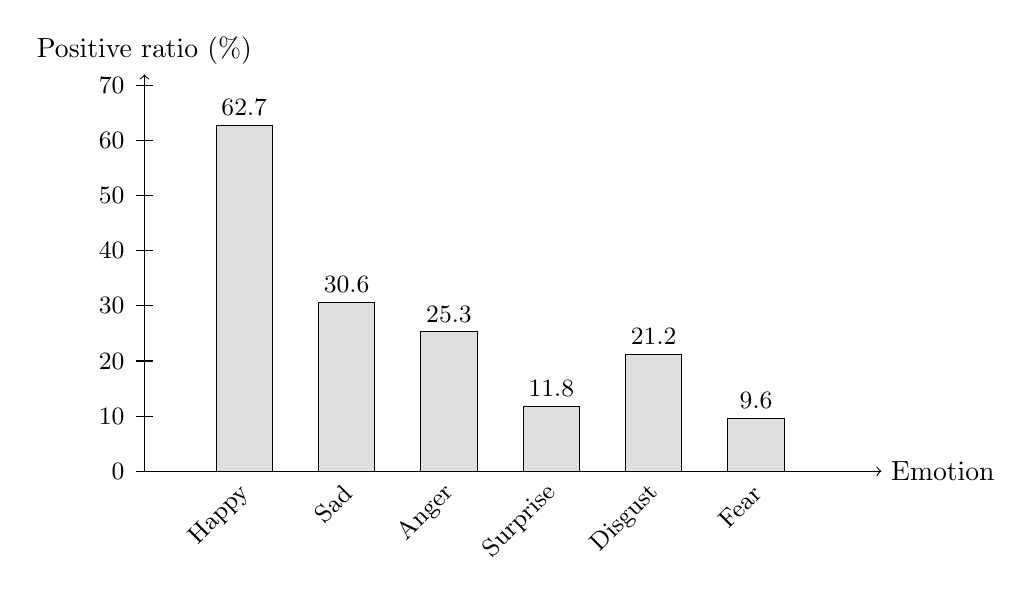
\begin{tikzpicture}[
    x=1.3cm,
    y=0.07cm
]

% Axes
\draw[->] (0,0) -- (7.2,0) node[right] {Emotion};
\draw[->] (0,0) -- (0,72) node[above] {Positive ratio (\%)};

% Y ticks
\foreach \y in {0,10,20,30,40,50,60,70} {
    \draw (-0.08,\y) -- (0.08,\y);
    \node[left] at (-0.1,\y) {\small \y};
}

% Bars: x, height, label
\foreach \x/\h/\name in {
    0.7/62.7/Happy,
    1.7/30.6/Sad,
    2.7/25.3/Anger,
    3.7/11.8/Surprise,
    4.7/21.2/Disgust,
    5.7/9.6/Fear
} {
    \draw[fill=gray!25] (\x,0) rectangle +(0.55,\h);
    \node[above, font=\small] at (\x+0.275,\h) {\h};
    \node[rotate=45, anchor=east, font=\small] at (\x+0.35,-2) {\name};
}

\end{tikzpicture}
\caption{Class imbalance in the filtered CMU-MOSEI six-emotion dataset.}
\label{fig:class_distribution}
\end{figure}

% ─────────────────────────────────────────────────────────────
\section{Multimodal Feature Preprocessing Pipeline}
\label{sec:data_collection}

The preprocessing pipeline converts CMU-MOSEI multimodal features into a fixed tensor format required by the neural network. The original dataset introduced by Zadeh et al. contains text, audio, visual information, and emotion annotations collected from online video segments \cite{zadeh2018multimodal}. In this work, preprocessing does not create a new dataset from participants. It prepares the existing features for training, validation, testing, and later prototype inference.

For the text stream, the available word-level information is converted into sentence-level input and processed with a frozen BERT-base-uncased model. The final representation is obtained by averaging the last four hidden layers of BERT. This produces a tensor of shape $[B, 50, 768]$, where $B$ is the batch size and 50 is the maximum sequence length. Before fusion, a linear projection maps this representation to the shared hidden dimension $[B, 50, 128]$.

\begin{equation}
H_{BERT} = \frac{H^{(9)} + H^{(10)} + H^{(11)} + H^{(12)}}{4}
\end{equation}

For the audio stream, COVAREP descriptors are used. Each sequence contains 74-dimensional vectors over a fixed length of 60 time steps, producing a tensor of shape $[B, 60, 74]$. These values represent speech-related properties such as pitch, spectral characteristics, and voice quality. For the visual stream, OpenFace-style facial features are used. Each sequence contains 35-dimensional facial action unit descriptors over 60 frames, producing a tensor of shape $[B, 60, 35]$. Audio and visual sequences are padded when they are shorter than the required length, and all tensors are converted to 32-bit floating point format.

After preprocessing, the prepared samples are stored in a pickle file for efficient loading. Each item contains text, audio, and visual tensors, a six-dimensional binary emotion label vector, and padding masks for audio and visual sequences. These masks indicate which frames are real observations and which are padding. This storage format allows batches to be loaded consistently across all experiments.

The same general input structure is considered for the prototype pipeline. For new video input, the system can extract audio with \texttt{ffmpeg}, compute acoustic descriptors with \texttt{opensmile}, detect facial action units with \texttt{py-feat}, and transcribe speech using \texttt{faster-whisper}. The recognized text is then tokenized and processed through BERT. This deployment-oriented flow is designed so that inference data follows the same general format as the training samples.

\begin{equation}
y_t = \sum_{i=0}^{k-1} w_i x_{t+i} + b
\end{equation}

% ── BEFORE: Raw CMU-MOSEI HDF5 ───────────────────────────────
\begin{table}[H]
\centering
\caption{CMU-MOSEI dataset statistics before preprocessing (raw HDF5 format).}
\label{tab:before_preprocessing}
\begin{tabular}{ll}
\hline
\textbf{Property} & \textbf{Value} \\
\hline
Format                        & HDF5 (.h5) \\
Total segments                & 23,453 \\
Splits                        & train / valid / test (fixed) \\
\hline
\multicolumn{2}{l}{\textit{Text modality}} \\
\hline
Field name                    & \texttt{words} \\
Representation                & Raw byte strings (word tokens) \\
Sequence length               & Variable (up to 50 words) \\
Dimension per token           & — (not embedded) \\
\hline
\multicolumn{2}{l}{\textit{Audio modality}} \\
\hline
Field name                    & \texttt{COVAREP} \\
Representation                & Float64 acoustic descriptors \\
Sequence length               & Variable (up to 500+ frames) \\
Dimension per frame           & 74 \\
\hline
\multicolumn{2}{l}{\textit{Visual modality}} \\
\hline
Field name                    & \texttt{OpenFace\_2} \\
Representation                & Float64 facial action units \\
Sequence length               & Variable \\
Dimension per frame           & 713 (full feature set) \\
\hline
\multicolumn{2}{l}{\textit{Labels}} \\
\hline
Field name                    & \texttt{All Labels} \\
Format                        & Float scores per emotion \\
Emotions                      & happy, sad, anger, surprise, disgust, fear \\
Samples with all-zero labels  & 3,013 (excluded) \\
\hline
\multicolumn{2}{l}{\textit{Emotion distribution (train split, raw)}} \\
\hline
Happy    & 10,752 positive samples (38\%) \\
Sadness  & 5,601  positive samples (20\%) \\
Anger    & 4,600  positive samples (16\%) \\
Disgust  & 3,755  positive samples (13\%) \\
Surprise & 2,055  positive samples (7\%) \\
Fear     & 1,803  positive samples (6\%) \\
\hline
\end{tabular}
\end{table}
 
% ── AFTER: Preprocessed PKL ──────────────────────────────────
\begin{table}[H]
\centering
\caption{Dataset statistics after preprocessing (stored as \texttt{.pkl}).}
\label{tab:after_preprocessing}
\begin{tabular}{ll}
\hline
\textbf{Property} & \textbf{Value} \\
\hline
Format                        & Python pickle (.pkl) \\
\hline
\multicolumn{2}{l}{\textit{Split sizes after all-zero filtering}} \\
\hline
Train                         & 13,934 samples \\
Validation                    & 1,569  samples \\
Test                          & 3,957  samples \\
\hline
\multicolumn{2}{l}{\textit{Text modality}} \\
\hline
Fields                        & \texttt{input\_ids}, \texttt{attention\_mask} \\
Representation                & BERT-base-uncased tokenization \\
Sequence length               & Fixed 50 tokens (padded / truncated) \\
Dtype                         & int64 \\
Shape per sample              & $[50]$ \\
\hline
\multicolumn{2}{l}{\textit{Audio modality}} \\
\hline
Field                         & \texttt{audio} \\
Representation                & COVAREP, z-normalized, resampled \\
Sequence length               & Fixed 60 frames \\
Dimension per frame           & 74 \\
Dtype                         & float32 \\
Shape per sample              & $[60, 74]$ \\
\hline
\multicolumn{2}{l}{\textit{Visual modality}} \\
\hline
Field                         & \texttt{vision} \\
Representation                & OpenFace AU subset, z-normalized \\
Sequence length               & Fixed 60 frames \\
Dimension per frame           & 35 \\
Dtype                         & float32 \\
Shape per sample              & $[60, 35]$ \\
\hline
\multicolumn{2}{l}{\textit{Labels}} \\
\hline
Field                         & \texttt{labels} \\
Format                        & Binary float32 vector \\
Shape per sample              & $[6]$ \\
Threshold applied             & score $> 0$ → label = 1 \\
\hline
\multicolumn{2}{l}{\textit{Positive class weights (BCEWithLogitsLoss)}} \\
\hline
Happy    & 0.60 \\
Sad      & 2.26 \\
Anger    & 2.95 \\
Surprise & 7.49 \\
Disgust  & 3.72 \\
Fear     & 9.47 \\
\hline
\end{tabular}
\end{table}

% ============================================================
% Figure: modality_dropout.tex
% ============================================================

\begin{figure}[H]
\centering
\resizebox{0.95\textwidth}{!}{%
\begin{tikzpicture}[
    node distance=0.6cm and 1.0cm,
    tblock/.style={
        rectangle, rounded corners=4pt, align=center,
        minimum width=2.7cm, minimum height=0.75cm, font=\small,
        fill=colText!18, draw=colText!70, line width=0.8pt
    },
    ablock/.style={
        rectangle, rounded corners=4pt, align=center,
        minimum width=2.7cm, minimum height=0.75cm, font=\small,
        fill=colAudio!18, draw=colAudio!70, line width=0.8pt
    },
    vblock/.style={
        rectangle, rounded corners=4pt, align=center,
        minimum width=2.7cm, minimum height=0.75cm, font=\small,
        fill=colVision!18, draw=colVision!70, line width=0.8pt
    },
    zblock/.style={
        rectangle, rounded corners=4pt, align=center,
        minimum width=2.7cm, minimum height=0.75cm, font=\small,
        fill=gray!12, draw=gray!55, line width=0.8pt, dashed
    },
    mblock/.style={
        rectangle, rounded corners=5pt, align=center,
        minimum width=2.3cm, minimum height=2.0cm, font=\small,
        fill=colBottle!15, draw=colBottle!70, line width=1.0pt
    },
    lblock/.style={
        rectangle, rounded corners=4pt, align=center,
        minimum width=2.1cm, minimum height=0.7cm, font=\scriptsize,
        fill=colFuse!12, draw=colFuse!60, line width=0.7pt
    },
    note/.style={
        font=\scriptsize, align=center, text=gray!70
    },
    title/.style={
        font=\small\sffamily\bfseries, align=center, text=colArrow
    },
    tarrT/.style={-{Stealth[length=4pt]}, line width=0.8pt, color=colText!80},
    tarrA/.style={-{Stealth[length=4pt]}, line width=0.8pt, color=colAudio!80},
    tarrV/.style={-{Stealth[length=4pt]}, line width=0.8pt, color=colVision!80},
    tarrZ/.style={-{Stealth[length=3.5pt]}, line width=0.7pt, dashed, color=gray!60},
    tarrB/.style={-{Stealth[length=4pt]}, line width=0.8pt, color=colBottle!80}
]

% ---------------- Left side: normal pass ----------------
\node[title] (titleL) at (0,0) {Normal forward pass};

\node[tblock] (tL) at (0,-1.0) {Text\\$[B,50,128]$};
\node[ablock] (aL) at (0,-2.0) {Audio\\$[B,60,74]$};
\node[vblock] (vL) at (0,-3.0) {Vision\\$[B,60,35]$};

\node[mblock] (mL) at (3.3,-2.0) {Bottleneck\\Fusion};
\node[lblock] (oL) at (6.0,-2.0) {6 logits};

\draw[tarrT] (tL.east) -- (mL.west);
\draw[tarrA] (aL.east) -- (mL.west);
\draw[tarrV] (vL.east) -- (mL.west);
\draw[tarrB] (mL.east) -- (oL.west);

\node[note] at (0,-3.75) {all modalities active};

% ---------------- Separator ----------------
\node[font=\Large, text=gray!55, align=center] at (7.5,-2.0) {$\Longrightarrow$};
\node[note] at (7.5,-2.75) {$p=0.05$\\independent};

% ---------------- Right side: dropout pass ----------------
\node[title] (titleR) at (11.2,0) {Modality dropout};

\node[tblock] (tR) at (11.2,-1.0) {Text\\$[B,50,128]$};
\node[zblock] (aR) at (11.2,-2.0) {Audio\\$\rightarrow$ zeros};
\node[vblock] (vR) at (11.2,-3.0) {Vision\\$[B,60,35]$};

\node[mblock] (mR) at (14.5,-2.0) {Bottleneck\\Fusion};
\node[lblock] (oR) at (17.2,-2.0) {6 logits};

\draw[tarrT] (tR.east) -- (mR.west);
\draw[tarrZ] (aR.east) -- (mR.west);
\draw[tarrV] (vR.east) -- (mR.west);
\draw[tarrB] (mR.east) -- (oR.west);

\node[note] at (11.2,-3.75) {audio stream replaced with zeros};

\end{tikzpicture}%
}
\caption{Modality dropout applied during training. With probability $p=0.05$, one non-text modality can be replaced with zeros independently. This regularisation reduces dependence on a single input stream and improves robustness during multimodal fusion.}
\label{fig:modality_dropout}
\end{figure}
% ─────────────────────────────────────────────────────────────
% ─────────────────────────────────────────────────────────────
\section{Evaluation Metrics, Training Protocol, and Ablation Design}
\label{sec:data_analysis}

The experimental analysis follows three stages. First, the study evaluates the trained models on the test set using standard classification metrics. Second, it compares ablation configurations to measure the effect of individual design choices. Third, it tunes class-specific decision thresholds on the validation set and applies them during final testing.

Macro-averaged F1-score serves as the primary metric. This metric calculates the mean F1-score across the six emotion categories and gives equal importance to each class. This choice matters for CMU-MOSEI because frequent emotions can dominate general accuracy. The study also reports average weighted accuracy as a secondary measure, since it considers the balance between positive and negative predictions for each category. In addition, per-class F1-scores show how well the system recognises each emotion separately. Pan et al. also emphasise class-level analysis in multimodal emotion recognition, because aggregated scores can hide weak results for specific categories \cite{pan2023multimodal}.

\textbf{For each class, the evaluation is based on true positives (TP), false positives (FP), and false negatives (FN).}

Precision is defined as:
\begin{equation}
Precision = \frac{TP}{TP + FP}
\end{equation}

Recall is defined as:
\begin{equation}
Recall = \frac{TP}{TP + FN}
\end{equation}

The F1-score is the harmonic mean of precision and recall:
\begin{equation}
F1 = \frac{2 \cdot Precision \cdot Recall}{Precision + Recall}
\end{equation}

Macro-F1 is computed as:
\begin{equation}
Macro\text{-}F1 = \frac{1}{C} \sum_{i=1}^{C} F1_i
\end{equation}

where $C$ is the number of emotion classes.

Weighted accuracy is defined as:
\begin{equation}
Weighted\ Accuracy = \frac{\sum_{i=1}^{C} w_i \cdot TP_i}{\sum_{i=1}^{C} w_i \cdot N_i}
\end{equation}

where $w_i$ is the weight of class $i$, and $N_i$ is the number of samples in class $i$.

In addition, per-class F1-scores show how well the system recognises each emotion separately.

The training process handles class imbalance with weighted binary cross-entropy loss. Each emotion receives a positive weight based on the ratio between negative and positive samples in the training split. As a result, rare categories create a stronger learning signal during backpropagation. Figure~\ref{fig:positive_weights} presents the computed positive weights. Fear and surprise receive the largest values because they appear less often in the dataset.

\begin{equation}
\mathcal{L}_{BCE} =
- \left[
y \log(\sigma(x)) +
(1-y)\log(1-\sigma(x))
\right]
\end{equation}

\begin{figure}[H]
\centering
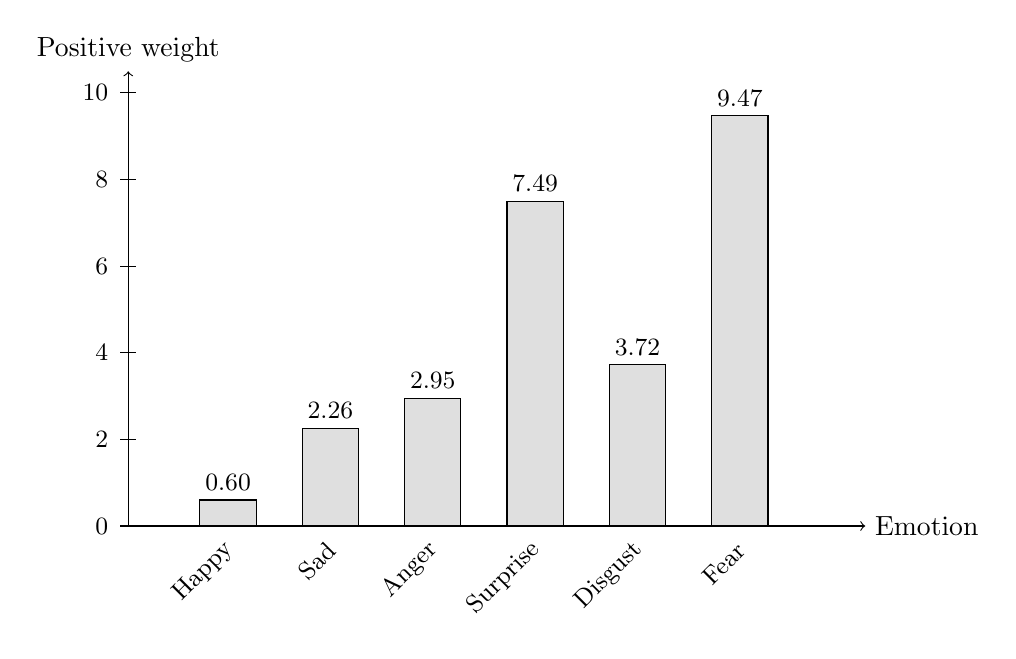
\begin{tikzpicture}[
    x=1.3cm,
    y=0.55cm
]

% Axes
\draw[->] (0,0) -- (7.2,0) node[right] {Emotion};
\draw[->] (0,0) -- (0,10.5) node[above] {Positive weight};

% Y ticks
\foreach \y in {0,2,4,6,8,10} {
    \draw (-0.08,\y) -- (0.08,\y);
    \node[left] at (-0.1,\y) {\small \y};
}

% Bars
\foreach \x/\h/\name in {
    0.7/0.60/Happy,
    1.7/2.26/Sad,
    2.7/2.95/Anger,
    3.7/7.49/Surprise,
    4.7/3.72/Disgust,
    5.7/9.47/Fear
} {
    \draw[fill=gray!25] (\x,0) rectangle +(0.55,\h);
    \node[above, font=\small] at (\x+0.275,\h) {\h};
    \node[rotate=45, anchor=east, font=\small] at (\x+0.35,-0.3) {\name};
}

\end{tikzpicture}
\caption{Class-specific positive weights used in BCEWithLogitsLoss.}
\label{fig:positive_weights}
\end{figure}

Figure~\ref{fig:training_protocol} summarises the training procedure. The models use the AdamW optimiser with a learning rate of $10^{-4}$ and cosine annealing. Gradient clipping with a maximum norm of 1.0 reduces unstable updates. Training runs for at most 50 epochs, and early stopping monitors validation macro-F1 with a patience of 10 epochs. The BERT encoder remains frozen during training. Modality dropout with probability $p = 0.05$ affects the audio and visual streams independently.

\begin{equation}
Attention(Q,K,V)=softmax\left(\frac{QK^T}{\sqrt{d_k}}\right)V
\end{equation}

\begin{figure}[H]
\centering
\resizebox{\textwidth}{!}{
\begin{tikzpicture}[
    node distance=0.8cm and 0.75cm,
    block/.style={
        rectangle,
        draw,
        rounded corners=3pt,
        align=center,
        minimum width=2.4cm,
        minimum height=0.9cm,
        font=\small
    },
    arrow/.style={-Latex, thick}
]

\node[block] (data) {Filtered\\CMU-MOSEI};
\node[block, right=of data] (split) {Train / Valid / Test\\standard split};
\node[block, right=of split] (loss) {Weighted BCE\\+ auxiliary losses};
\node[block, right=of loss] (optim) {AdamW\\cosine annealing};
\node[block, right=of optim] (early) {Early stopping\\validation Macro-F1};
\node[block, right=of early] (test) {Test evaluation\\Macro-F1 + Avg.WA};

\node[block, below=1.2cm of early] (threshold) {Per-class threshold tuning\\on validation set};

\draw[arrow] (data) -- (split);
\draw[arrow] (split) -- (loss);
\draw[arrow] (loss) -- (optim);
\draw[arrow] (optim) -- (early);
\draw[arrow] (early) -- (test);

\draw[arrow] (early) -- (threshold);
\draw[arrow] (threshold) -| (test);

\end{tikzpicture}
}
\caption{Training and evaluation protocol used in the experimental study.}
\label{fig:training_protocol}
\end{figure}

The ablation study includes eight experimental configurations. Each configuration changes one specific part of the architecture or training strategy, such as BERT freezing, the number of averaged hidden layers, auxiliary losses, modality dropout, or threshold tuning. All experiments use the same split, preprocessing pipeline, and training settings. This setup links changes in macro-F1, weighted accuracy, and per-class F1 to the tested component.

The study performs threshold tuning after training. For each emotion, the decision threshold varies from 0.10 to 0.90 with a step of 0.05. The validation set selects the threshold that gives the highest F1-score for each class. The final test stage then uses these thresholds, and the results also include the default threshold value of 0.5 for comparison.

\begin{equation}
\hat{y} =
\begin{cases}
1, & p \ge t \\
0, & p < t
\end{cases}
\end{equation}

% ─────────────────────────────────────────────────────────────
% ─────────────────────────────────────────────────────────────
% ─────────────────────────────────────────────────────────────
% ─────────────────────────────────────────────────────────────
\section{Limitations of the Research Approach}
\label{sec:limitations}

Several limitations should guide the interpretation of the experimental results. The first limitation concerns the input representations. COVAREP and OpenFace-style descriptors provide compact and interpretable signals, but they contain less information than modern neural audio and visual encoders. For example, systems that use VGGish or ResNet18 can extract richer modality representations than handcrafted descriptors. Therefore, this study shows what the selected feature format and architecture can achieve, not the maximum possible performance of bottleneck fusion in general. Koromilas and Giannakopoulos also note that feature representation quality strongly affects results in multimodal emotion recognition \cite{koromilas2021deep}.

The second limitation concerns language and cultural scope. CMU-MOSEI mainly contains English-language speech from online videos. The study does not evaluate the trained system on other languages, accents, or cultural communication styles. For this reason, its generalisation to multilingual or culturally diverse settings remains uncertain.

Another limitation concerns inference time in the prototype pipeline. Processing a short video may require several seconds because the system needs to extract audio features, detect facial action units, transcribe speech, and run the neural network. This speed suits a research prototype, but it does not yet support real-time interaction.

Finally, the experiments use a fixed dataset split. This keeps the comparison consistent, but it does not test performance across different speaker groups, recording conditions, or datasets. This work does not include cross-dataset evaluation.

% ─────────────────────────────────────────────────────────────
% ─────────────────────────────────────────────────────────────
\section{Validity and Reliability of Experimental Results}
\label{sec:validity}

The study uses several measures to keep the experimental results consistent and reproducible. A fixed random seed of 42 controls random variation from weight initialisation and data loading. All ablation configurations use the same train, validation, and test split, the same preprocessing pipeline, and the same evaluation code. This setup helps ensure that the observed differences come from the tested design choices rather than inconsistent experimental conditions.

CMU-MOSEI supports external validity because many studies use it for multimodal emotion and sentiment analysis. Its video segments come from real online sources, so it reflects more natural communication than small laboratory datasets with acted emotions. The training process never uses the test set for model selection or threshold tuning. This separation helps the final results reflect generalisation to unseen samples.

Standard metrics also support reliability. The study calculates macro-F1, weighted accuracy, and per-class F1 in the same way for all configurations. Ramyasree et al. note that shared evaluation protocols help researchers compare multimodal emotion recognition models fairly \cite{ramyasree2025emotion}. Recent graph-based work also stresses that ablation variants need identical testing conditions to support reliable conclusions about individual components \cite{anonymous2026context}.

% ─────────────────────────────────────────────────────────────
% ─────────────────────────────────────────────────────────────
\section{Ethical Considerations in Multimodal Emotion Recognition}
\label{sec:ethics}

The ethical aspect of this work concerns both the dataset and the possible use of emotion recognition technology. Zadeh et al. created CMU-MOSEI from publicly available YouTube videos for academic research purposes \cite{zadeh2018multimodal}. This study does not collect new personal data, recruit participants, or create additional annotations. The experiments use only the prepared dataset and its feature representations.

The MultiMOOD prototype functions as a research demonstration. The system processes submitted video files for inference and should not store them permanently. The pipeline should remove temporary files after processing and should not retain audio, video, or transcript data after prediction. This design reduces privacy risks and keeps users in control of submitted content.

A broader concern involves demographic and cultural bias. Kalateh et al. explain that emotion recognition systems may behave unevenly when training data mostly represents one language, culture, or recording context \cite{kalateh2024systematic}. Since CMU-MOSEI mainly contains English-speaking online videos, the trained system may not work equally well for speakers with different accents, backgrounds, or expression styles. Any use beyond the academic setting should consider this limitation carefully.

Emotion recognition also raises concerns about consent and surveillance. The prototype does not target hidden monitoring or decision-making about individuals. Any future deployment would need explicit consent, a transparent explanation of the prediction process, and clear limits on how users or institutions may use the outputs. This project treats the technology as an experimental tool rather than a final decision-making system.

% ─────────────────────────────────────────────────────────────
\section{Mathematical Representation of the Applied Models}
\label{sec:model_formulations}

This section summarises the main neural architectures and mathematical operations used in the proposed multimodal emotion recognition system. The implemented model combines BERT-based text representations, convolutional feature extraction, bidirectional sequence modelling, and transformer attention mechanisms for multimodal fusion.

The text modality is processed using the BERT-base-uncased transformer encoder. The final sentence representation is obtained by averaging the last four hidden layers:

\begin{equation}
H_{BERT} =
\frac{
H^{(9)} + H^{(10)} + H^{(11)} + H^{(12)}
}{4}
\end{equation}

where $H^{(i)}$ denotes the hidden representation produced by the $i$-th BERT layer.

The transformer attention mechanism used inside BERT and the bottleneck fusion module is defined as:

\begin{equation}
Attention(Q,K,V)
=
softmax
\left(
\frac{QK^T}{\sqrt{d_k}}
\right)V
\end{equation}

where $Q$, $K$, and $V$ represent query, key, and value matrices.

Audio and visual streams are projected into the shared hidden space using one-dimensional convolutional layers. The convolution operation is defined as:

\begin{equation}
y_t =
\sum_{i=0}^{k-1}
w_i x_{t+i}
+
b
\end{equation}

where $x$ is the input sequence, $w_i$ are convolution kernel weights, $k$ is the kernel size, and $b$ is the bias term.

The architecture also uses bidirectional sequence modelling. In a BiLSTM layer, forward and backward hidden states are concatenated:

\begin{equation}
h_t =
\overrightarrow{LSTM}(x_t)
\oplus
\overleftarrow{LSTM}(x_t)
\end{equation}

where $\oplus$ denotes vector concatenation.

Cross-modal interaction follows the same principle as the MulT transformer architecture, where one modality attends to another through cross-attention:

\begin{equation}
Attention_{A \rightarrow T}(Q_A,K_T,V_T)
=
softmax
\left(
\frac{Q_AK_T^T}{\sqrt{d_k}}
\right)V_T
\end{equation}

where the audio modality attends to textual representations.

The final training objective uses weighted binary cross-entropy loss:

\begin{equation}
\mathcal{L}_{BCE} =
-
\left[
y\log(\sigma(x))
+
(1-y)\log(1-\sigma(x))
\right]
\end{equation}

where $y$ is the ground-truth label, $x$ is the predicted logit, and $\sigma(x)$ is the sigmoid activation function.

During inference, class-specific thresholds are applied to convert probabilities into binary predictions:

\begin{equation}
\hat y =
\begin{cases}
1, & p \ge t \\
0, & p < t
\end{cases}
\end{equation}

where $p$ is the predicted probability and $t$ is the selected decision threshold.